\begin{enumerate}[label=\thesubsection.\arabic*,ref=\thesubsection.\theenumi]
  \item For which values of $a$ and $b$ does the following pair of linear equations have an infinite number of solutions?
	\begin{align}
		2x+3y&=7\\
		(a-b)x+(a-b)y&=3a+b-2
	\end{align}
  \item For which value of $k$ will the following pair of linear equations have no solution?
	\begin{align}
		3x+y&=1\\
		(2k-1)x+(k-1)y&=2k+1
	\end{align}
\item Find the values of $k$ for which the line 
\begin{align}
(k-3)x-(4-k^2)y+k^2-7k+6=0 \label{eq:chapters/11/10/4/1/1}
\end{align}
is
\begin{enumerate}
\item Parallel to the $x$-axis
\item Parallel to the $y$-axis
\item Passing through the origin
\end{enumerate}
    \solution 
		The parameters of the given line are
\begin{align}
\vec{n}^{\top}\vec{x}=c \label{eq:chapters/11/10/4/1/2}
\end{align}
This equation can be expressed in the form of 
\begin{align}
\vec{n} = \myvec{k-3\\-4+k^2}, c  = -k^2+7k-6
\end{align}
\iffalse
Then \eqref{eq:chapters/11/10/4/1/1} can be expressed as
\begin{align}
\myvec{k-3 & -4+k^2}\vec{x} &=-k^2+7k-6\label{eq:chapters/11/10/4/1/4}
\end{align}
\fi
\begin{enumerate}
%part-1
    \item 
	    In this case,
	    \iffalse
The normal vector of $x$-axis is given by
\begin{align}
\myvec{0\\1}
\end{align}
\fi
equating $\vec{n}$ to the normal vector of $x$-axis,
\begin{align}
\myvec{k-3\\-4+k^2} &=\alpha\myvec{0\\1}\label{eq:chapters/11/10/4/1/6}
\\
\implies
k &=3
\end{align}
Substituting the value of $k$ in \eqref{eq:chapters/11/10/4/1/1}, the desired equation is
\begin{align}
        \myvec{0 & 5}\vec{x} &=6
\end{align}

\item In this case, 
equating $\vec{n}$ to the normal vector of $y$-axis,
\begin{align}
\myvec{k-3\\-4+k^2} &=\beta\myvec{1\\0}\label{eq:chapters/11/10/4/1/11}
\\
	\implies k &=\pm2
\end{align}
Substituting the value of $k$ in \eqref{eq:chapters/11/10/4/1/1}, the desired equation is 
\begin{align}
        \myvec{-1 & 0}\vec{x} &=4, \quad  k &=2\\
        \myvec{-5 & 0}\vec{x} &=-24, \quad  k &=-2
\end{align}
\item 
	In this case, 
\begin{align}
	c = 0 \implies 
	-k^2+7k-6 &= 0\\
	\implies k =1 \text{ or } k&=6
\end{align}
Substituting the value of $k$ in \eqref{eq:chapters/11/10/4/1/1}, the desired equations are 
\begin{align}
        \myvec{-2 & -3}\vec{x} &=0, \quad  k &=1\\
       \myvec{3 & 32}\vec{x} &=0, \quad  k &=6
\end{align}
\end{enumerate}

	\item Find the  equations of the lines, which cutoff intercepts on the axes  whose sum and product are 1 and -6 respectively.
\\
\solution
		Let the intercepts be $a$ and  $b$. Then
\begin{align}
a+b=1,
ab=-6 \label{eq:11/10/4/32a}
\\
\implies  a = 3, b = -2
\end{align}
Thus, the possible 
intercepts are
\begin{align}
\myvec{3\\0}, \myvec{0\\-2},
\myvec{-2\\0}, \myvec{0\\3}
\end{align}
From
		\eqref{prop:lin-eq-unit-mat},
\begin{align}
	\myvec{3 & 0 \\ 0 &-2}\vec{n} = \myvec{1 \\ 1}
	\\
	\implies \vec{n} = \myvec{\frac{1}{3} \\ -\frac{1}{2}}
	\\
	\text{or, } \myvec{2 & -3}\vec{x} = 6
\end{align}
using		\eqref{prop:lin-eq-unit}.
Similarly, the other line can be obtained
as
\begin{align}
	\myvec { 3 & -2 }  \vec{x}  = -6        
\end{align}
See  
\figref{fig:11/10/4/3line segmenta}.
\begin{figure}[!htbp]
\centering
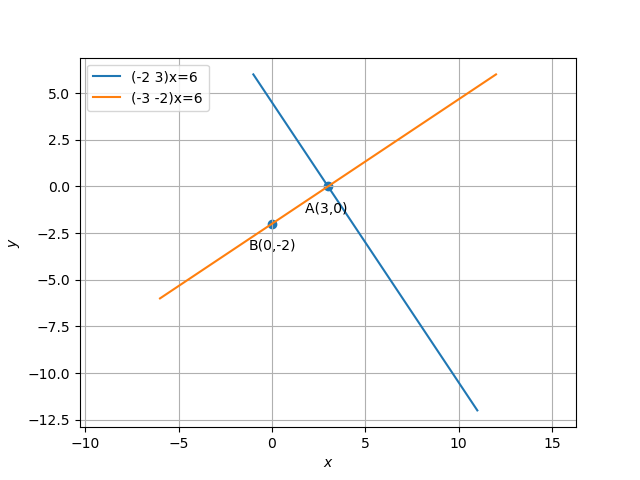
\includegraphics[width=\columnwidth]{chapters/11/10/4/3/figs/inter.png}
\caption{}
\label{fig:11/10/4/3line segmenta}
\end{figure}

\item A ray of light passing through the point $\vec{P} = \brak{1, 2}$ reflects on the x-axis at point $\vec{A}$ and the reflected ray passes through the point $\vec{Q} =\brak{5, 3}$. Find the coordinates of $\vec{A}$.
\\
    \solution 
			From \eqref{eq:11/10/4/22},
the reflection of $\vec{Q}$ is 
\begin{align}
\vec{R}  
= \myvec{5\\-3}
\end{align}
Letting
\begin{align}
\vec{A} = \myvec{x\\0},
\end{align}
since 
$\vec{P},
\vec{A},  
\vec{R}  
$
are collinear, 
		from \eqref{prop:lin-dep-rank},
\begin{align}
	\myvec{
		1 & 1 & 2 
		\\ 
		1 & 5 & -3 
		\\
		1 & x & 0 }
	\xleftrightarrow[R_3=R_3 - R_1]{R_2 = R_2 - R_1}
	\myvec{
		1 & 1 & 2 
		\\ 
		0 & 4 & -5 
		\\
		0 & x-1 & -2 }
	\\
	\xleftrightarrow[]{R_3 = 4R_3 - \brak{x-1}R_2}
	\myvec{
		1 & 1 & 2 
		\\ 
		0 & 4 & -5 
		\\
		0 & 0 & 5x-13 }
	\implies x = \frac{13}{5}
\end{align}
See  
\figref{fig:chapters/11/10/4/22/1}.
\begin{figure}[H]
\centering
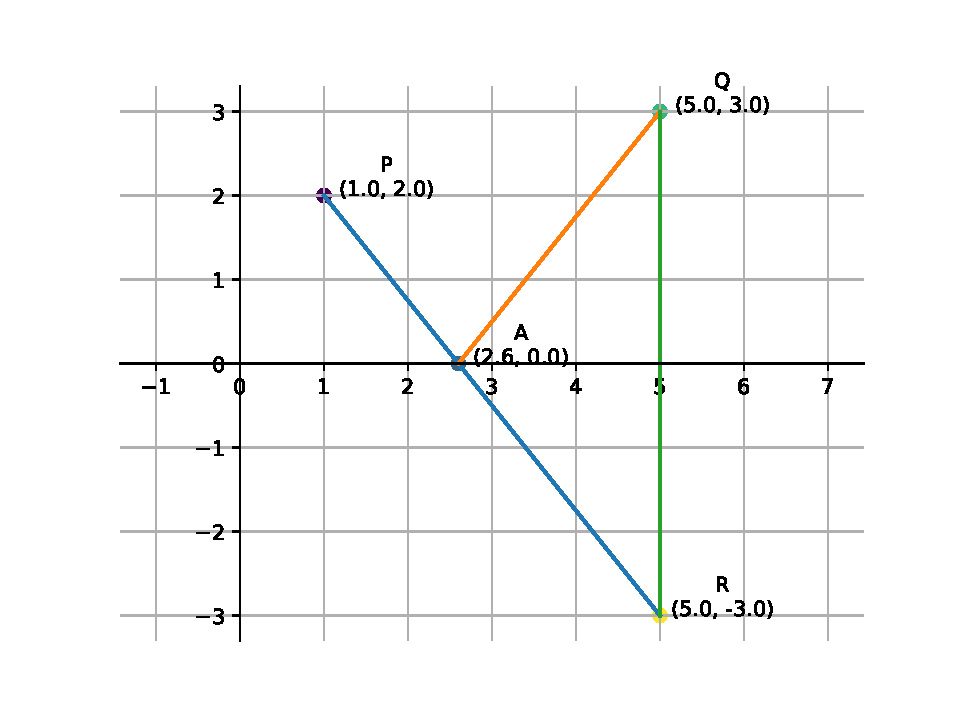
\includegraphics[width=0.75\columnwidth]{chapters/11/10/4/22/figs/fig.pdf}
\caption{}
\label{fig:chapters/11/10/4/22/1}
\end{figure}




\item The length $L$ in centimetre of a copper rod is a linear function of its celsius temperature $C$. In an experiment, if $L=124.942$. When $C=20$  and $L=125.134$. When $C=110$, express $L$ in terms of $C$.
\item The owner of a milk store finds that, he can sell $980$ litres of milk each week at \rupee~14/litre and $1220$ litres of milk each week at \rupee~16/litre. Assuming a linear relationship between selling price and demand, how many litres could he sell weekly at \rupee~17/ litre?
\item Prove that in any $\triangle{ABC}$, cos A=$\frac{b^2+c^2-a^2}{2bc}$, where a,b,c are the magnitudes of the sides opposite to the vertices A,B,C respectively.
\item Distance of the point $(\alpha, \beta, \gamma)$ from y-axis is
\begin{enumerate}
	\item $\beta$ 
	\item $\abs{\beta}$
	\item $\abs{\beta+\gamma}$
	\item $\sqrt{\alpha^2+\gamma^2}$
\end{enumerate}
\item The reflection of the point $(\alpha, \beta, \gamma )$ in the xy-plane is 
\begin{enumerate}
	\item $\alpha,\beta,0)$
	\item $(0,0,\gamma)$
	\item $(-\alpha,-\beta,\gamma)$
	\item $(\alpha,\beta,-\gamma)$
\end{enumerate}
\item The plane $ax+by=0$ is rotated about its line of intersection with the plane $z=0$ through an angle $\alpha.$ Prove that the equation of the plane in its new position is 
\begin{align*}
	ax+by \pm (\sqrt{a^2+b^2} \tan\alpha)z=0.
\end{align*}
\item The locus represented by $xy+yz=0$ is 
\begin{enumerate}
	\item A pair of perpendicular lines
	\item A pair of parallel lines
	\item A pair of parallel planes 
	\item A pair of perpendicular planes
\end{enumerate}
\item For what values of $a$ and $b$ the intercepts cut off on the coordinate axes by the line $ax+by+8=0$ are equal in length but opposite in signs to those cut off by the line $2x-3y=0$ on the axes.
\item If the equation of the base of an equilateral triangle is $x+y=2$ and the vertex is (2,-1), then find the length of the side of the triangle. 
\item A variable line passes through a fixed point $\vec{P}$. The algebraic sum of the perpendiculars drawn from the points (2,0), (0,2) and (1,1) on the line is zero. Find the coordinates of the point $\vec{P}$.  
\item A straight line moves so that the sum of the reciprocals of its intercepts made on axes is constant. Show that the line passes through a fixed point. 
\item If the sum of the distances of a moving point in a plane from the axes is $l$, then finds the locus of the point.  
\item $\vec{P}_1,\vec{P}_2$ are points on either of the two lines $y-\sqrt{3}\abs{x}=2$ at a distance of 5 units from their point of intersection. Find the coordinates of the root of perpendiculars drawn from $P_1, P_2$ on the bisector of the angle between the given lines.
\item If $p$ is the length of perpendicular from the origin on the lien $\frac{x}{a}+\frac{y}{b}=1$ and $a^2,p^2,b^2$ are in A.P, then show that $a^4+b^4=0$.
\item The point (4,1) undergoes the following two successive transformations :
\begin{enumerate}
\item Reflection about the line $y=x$
\item Translation through a distance 2 units along the positive $x$-axis 
\end{enumerate}
Then the final coordinates of the point are
\begin{enumerate}
\item (4,3)
\item (3,4)
\item (1,4)
\item $\frac{7}{2}$,$\frac{7}{2}$
\end{enumerate}
\item One vertex of the equilateral with centroid at the origin and one side as $x+y-2=0$ is
\begin{enumerate}
\item (-1,-1)
\item (2,2)
\item (-2-2)
\item (2,-2)
\end{enumerate}
\item If $a,b,c$ are is A.P., then the straight lines $ax+by+c=0$ will always pass through \rule{1cm}{0.15mm}.
\item The points (3,4) and (2,-6) are situated on the \rule{1cm}{0.15mm} of the line $3x-4y-8=0$.
\item A point moves so that square of its distance from the point (3,-2) is numerically equal to its distance from the line $5x-12y=3$. The equation of its locus is %\rule{1cm}{0.15mm}.
\item Locus of the mid-points of the portion of the line $x\sin\theta+y\cos\theta=p$ intercepted between the axes is \rule{1cm}{0.15mm}.

State whether the following statements are true or false. Justify.
\item If the vertices of a triangle have integral coordinates, then the triangle can not be equilateral.
\item The line $\frac{x}{a}+\frac{y}{b}=1$ moves in such a way that $\frac{1}{a^2}+\frac{1}{b^2}=\frac{1}{c^2}$, where $c$ is a constant. The locus of the foot of the perpendicular from the origin on the given line is $x^2+y^2=c^2$.
\item 
Match the following
	\begin{table}[H]
\centering
	\resizebox{\columnwidth}{!}{
\begin{matchtabular}
  The coordinates of the points P and Q on the line x + 5y = 13 which are at a distance of 2 units from the line 12x – 5y + 26 = 0 are & (3,1),(-7,11)\\
  The coordinates of the point on the line x + y = 4, which are at a unit distance from the line 4x + 3y – 10 = 0 are & $-\frac{1}{11},\frac{11}{3}$ , $\frac{4}{3},\frac{7}{3}$\\
  The coordinates of the point on the line joining A (–2, 5) and B (3, 1) such that AP = PQ = QB are & 1,$\frac{12}{5}$ , $-3,\frac{16}{5}$\\
\end{matchtabular}
		}
		\caption{}
		\label{tab:lin-misc-1}
	\end{table}
\item The value of the $\lambda$, if the lines\\$(2x+3y+4)+\lambda(6x-y+12)=0$ are
	\begin{table}[H]
\centering
	\resizebox{\columnwidth}{!}{
\begin{matchtabular}
parallel to $y$-axis is & $\lambda =-\frac{3}{4}$\\
perpendicular to $7x+y-4=0$ is & $\lambda=-\frac{1}{3}$\\
passes through (1,2) is & $\lambda=-\frac{17}{41}$\\
parallel to $x$ axis is & $\lambda=3$\\
\end{matchtabular}
		}
		\caption{}
		\label{tab:lin-misc-2}
	\end{table}
\item The equation of the line through the intersection of the lines $2x-3y=0$ and $4x-5y=2$ and
	\begin{table}[H]
\centering
	\resizebox{\columnwidth}{!}{
\begin{matchtabular}
through the point (2,1) is & $2x-y=4$\\
perpendicular to the line & $x+y-5=0$\\
parallel to the line $3x-4y+5=0$ is & $x-y-1=0$\\
equally inclined to the axes is & $3x-4y-1=0$\\
\end{matchtabular}
		}
		\caption{}
		\label{tab:lin-misc-3}
	\end{table}
\item Point $\vec{R}\brak{h, k}$ divides a line segment between the axes in the ratio 1: 2. Find the equation of the line.
\label{chapters/11/10/2/19}
	\\
	\solution 
\iffalse
\documentclass[journal,12pt,twocolumn]{IEEEtran}
\usepackage{setspace}
\usepackage{gensymb}
\singlespacing
\usepackage[cmex10]{amsmath}
\usepackage{amsthm}
\usepackage{mathrsfs}
\usepackage{txfonts}
\usepackage{stfloats}
\usepackage{bm}
\usepackage{cite}
\usepackage{cases}
\usepackage{subfig}
\usepackage{longtable}
\usepackage{multirow}
\usepackage{enumitem}
\usepackage{mathtools}
\usepackage{steinmetz}
\usepackage{tikz}
\usepackage{circuitikz}
\usepackage{verbatim}
\usepackage{tfrupee}
\usepackage[breaklinks=true]{hyperref}
\usepackage{tkz-euclide}
\usetikzlibrary{calc,math}
\usepackage{listings}
    \usepackage{color}                                            %%
    \usepackage{array}                                            %%
    \usepackage{longtable}                                        %%
    \usepackage{calc}                                             %%
    \usepackage{multirow}                                         %%
    \usepackage{hhline}                                           %%
    \usepackage{ifthen}                                           %%
  %optionally (for landscape tables embedded in another document): %%
    \usepackage{lscape}     
\usepackage{multicol}
\usepackage{chngcntr}
\DeclareMathOperator*{\Res}{Res}
\renewcommand\thesection{\arabic{section}}
\renewcommand\thesubsection{\thesection.\arabic{subsection}}
\renewcommand\thesubsubsection{\thesubsection.\arabic{subsubsection}}

\renewcommand\thesectiondis{\arabic{section}}
\renewcommand\thesubsectiondis{\thesectiondis.\arabic{subsection}}
\renewcommand\thesubsubsectiondis{\thesubsectiondis.\arabic{subsubsection}}

% correct bad hyphenation here
\hyphenation{op-tical net-works semi-conduc-tor}
\def\inputGnumericTable{}                                 %%

\lstset{
frame=single, 
breaklines=true,
columns=fullflexible
}

\begin{document}


\newtheorem{theorem}{Theorem}[section]
\newtheorem{problem}{Problem}
\newtheorem{proposition}{Proposition}[section]
\newtheorem{lemma}{Lemma}[section]
\newtheorem{corollary}[theorem]{Corollary}
\newtheorem{example}{Example}[section]
\newtheorem{definition}[problem]{Definition}
\newcommand{\BEQA}{\begin{eqnarray}}
\newcommand{\EEQA}{\end{eqnarray}}
\newcommand{\define}{\stackrel{\triangle}{=}}

\bibliographystyle{IEEEtran}
\providecommand{\mbf}{\mathbf}
\providecommand{\pr}[1]{\ensuremath{\Pr\left(#1\right)}}
\providecommand{\qfunc}[1]{\ensuremath{Q\left(#1\right)}}
\providecommand{\sbrak}[1]{\ensuremath{{}\left[#1\right]}}
\providecommand{\lsbrak}[1]{\ensuremath{{}\left[#1\right.}}
\providecommand{\rsbrak}[1]{\ensuremath{{}\left.#1\right]}}
\providecommand{\brak}[1]{\ensuremath{\left(#1\right)}}
\providecommand{\lbrak}[1]{\ensuremath{\left(#1\right.}}
\providecommand{\rbrak}[1]{\ensuremath{\left.#1\right)}}
\providecommand{\cbrak}[1]{\ensuremath{\left\{#1\right\}}}
\providecommand{\lcbrak}[1]{\ensuremath{\left\{#1\right.}}
\providecommand{\rcbrak}[1]{\ensuremath{\left.#1\right\}}}
\theoremstyle{remark}
\newtheorem{rem}{Remark}
\newcommand{\sgn}{\mathop{\mathrm{sgn}}}
\providecommand{\abs}[1]{\left\vert#1\right\vert}
\providecommand{\res}[1]{\Res\displaylimits_{#1}} 
\providecommand{\norm}[1]{\left\lVert#1\right\rVert}
\providecommand{\mtx}[1]{\mathbf{#1}}
\providecommand{\mean}[1]{E\left[ #1 \right]}
\providecommand{\fourier}{\overset{\mathcal{F}}{ \rightleftharpoons}}
\providecommand{\system}{\overset{\mathcal{H}}{ \longleftrightarrow}}
\newcommand{\solution}{\noindent \textbf{Solution: }}
\newcommand{\cosec}{\,\text{cosec}\,}
\providecommand{\dec}[2]{\ensuremath{\overset{#1}{\underset{#2}{\gtrless}}}}
\newcommand{\myvec}[1]{\ensuremath{\begin{pmatrix}#1\end{pmatrix}}}
\newcommand{\mydet}[1]{\ensuremath{\begin{vmatrix}#1\end{vmatrix}}}
\numberwithin{equation}{subsection}
\makeatletter
\@addtoreset{figure}{problem}
\makeatother

\let\StandardTheFigure\thefigure
\let\vec\mathbf
\renewcommand{\thefigure}{\theproblem}



\def\putbox#1#2#3{\makebox[0in][l]{\makebox[#1][l]{}\raisebox{\baselineskip}[0in][0in]{\raisebox{#2}[0in][0in]{#3}}}}
     \def\rightbox#1{\makebox[0in][r]{#1}}
     \def\centbox#1{\makebox[0in]{#1}}
     \def\topbox#1{\raisebox{-\baselineskip}[0in][0in]{#1}}
     \def\midbox#1{\raisebox{-0.5\baselineskip}[0in][0in]{#1}}

\vspace{3cm}


\title{Assignment 1}
\author{Jaswanth Chowdary Madala}





% make the title area
\maketitle

\newpage

%\tableofcontents

\bigskip

\renewcommand{\thefigure}{\theenumi}
\renewcommand{\thetable}{\theenumi}


\begin{enumerate}


\textbf{Solution:} 
\fi
		Let the line segment between the axes be $AB$, with point $\vec{A}$ on X-axis, $\vec{B}$ on Y-axis. Let the points $\vec{A}$, $\vec{B}$ be
\begin{align}
\vec{A} = \myvec{\alpha\\0}, \,\vec{B} = \myvec{0 \\ \beta}
\end{align}
Given that $\frac{AR}{RB} = \frac{1}{2}$. By using section formula, we get
%
\begin{align}
\vec{R} &= \dfrac{2\vec{A} + \vec{B}}{3} \\
\myvec{h\\k} &= \dfrac{1}{3}\myvec{2\alpha\\\beta} \\
h &= \dfrac{2\alpha}{3}\\
k &= \dfrac{\beta}{3}\\
\vec{A} = \myvec{\frac{3h}{2}\\0}, \ \vec{B} &= \myvec{0\\3k}
\end{align}
The direction vector of the line is given by,
\begin{align}
\vec{m} &= \vec{R} - \vec{B}\\
\vec{m} &= \myvec{h\\-2k}
\end{align}
%
The normal vector to the line is given by,
\begin{align}
\vec{n} &= \myvec{2k\\h}
\end{align}
%
The equation of the line is given by,
\begin{align}
\vec{n}^{\top}\vec{x} &= \vec{n}^{\top}\vec{B}\\
\implies \myvec{2k&h}\vec{x} &= \myvec{2k&h}\myvec{0\\3k}\\
	\text{or, }\myvec{2k&h}\vec{x} &= 3hk
\end{align}





\item The tangent of angle between the lines whose intercepts on the axes are $a,-b$ and $b,-a$, respectively, is
\begin{enumerate}
\item $\frac{a^2-b^2}{ab}$
\item $\frac{b^2-a^2}{2}$
\item $\frac{b^2-a^2}{2ab}$
\item none of these 
\end{enumerate}
\item Prove that the line through the point $(x_1,y_1)$ and parallel to the line $Ax+By+C=0$ is $A(x-x_1)+B(y-y_1)=0$.
\label{chapters/11/10/3/11}
\\
\solution
\iffalse
\documentclass[10pt]{article}
\usepackage{graphicx}
\usepackage[none]{hyphenat}
\usepackage{graphicx}
\usepackage{listings}
\usepackage[english]{babel}
\usepackage{siunitx}
\usepackage{graphicx}
\usepackage{caption} 
\usepackage{booktabs}
\usepackage{array}
\usepackage{amssymb} % for \because
\usepackage{amsmath}   % for having text in math mode
\usepackage{extarrows} % for Row operations arrows
\usepackage{listings}
\usepackage[utf8]{inputenc}
\lstset{
  frame=single,
  breaklines=true
}
\usepackage{hyperref}
  
%Following 2 lines were added to remove the blank page at the beginning
\usepackage{atbegshi}% http://ctan.org/pkg/atbegshi
\AtBeginDocument{\AtBeginShipoutNext{\AtBeginShipoutDiscard}}


%New macro definitions
\newcommand{\mydet}[1]{\ensuremath{\begin{vmatrix}#1\end{vmatrix}}}
\providecommand{\brak}[1]{\ensuremath{\left(#1\right)}}
\newcommand{\solution}{\noindent \textbf{Solution: }}
\newcommand{\myvec}[1]{\ensuremath{\begin{pmatrix}#1\end{pmatrix}}}
\providecommand{\norm}[1]{\left\lVert#1\right\rVert}
\providecommand{\abs}[1]{\left\vert#1\right\vert}
\let\vec\mathbf{}
\begin{document}

\begin{center}
\title{\textbf{STRAIGHT LINES}}
\date{\vspace{-5ex}} %Not to print date automatically
\maketitle
\end{center}

\section{11$^{th}$ Maths - Chapter 10}
This is Problem 11 from Exercise-10.3
\begin{enumerate}
\item Prove that the line through the point$(x_1,y_1)$ and parallel to the line A$x$+B$y$+C=0 is A$(x-x_1)$+B$(y-y_1)$=0.

\solution
Given 
\fi
The given line parameters are
\begin{align}
\vec{n}=\myvec{A\\B}, \, c = C
\end{align}
Let 
\begin{align}
\vec{P}=\myvec{x_1\\y_1}\\
\end{align}
Then the equation of the desired line is
\begin{align}
	\vec{n}^\top\brak{\vec{x}-\vec{P}}&=0\\
	\implies A(x-x_1)+B(y-y_1)&=0
\end{align}

\item  If ${p}$ and ${q}$ are the lengths of perpendiculars from the origin to the lines ${x}\cos\theta - {y}\sin\theta =  {k}\cos2\theta$ and ${x}\sec\theta + {y}\cosec\theta = {k}$, respectively, prove that ${p}^2 + 4{q}^2 = {k}^2$
\label{chapters/11/10/3/16}
\\
\solution
The line parameters are
\begin{align}
    \vec{n}_1 = \myvec{\cos\theta \\ -\sin\theta},  {c}_1 &= {k}\cos2\theta\\
    \vec{n}_2 = \myvec{\sin\theta \\ \cos\theta},  {c}_2 &= \frac{1}{2}{k}\sin2\theta
\end{align}
			From \eqref{eq:PQ-final},
\begin{align}
    {p} &= \frac{\abs{  \vec{n}_1^{\top}\vec{x}-{c}_1 }}{\norm{\vec{n}_1}} 
    = \abs{{k}\cos2\theta} \\
     {q} &= \frac{\abs{  \vec{n}_2^{\top}\vec{x}-{c}_2 }}{\norm{\vec{n}_2}} 
    = \abs{ \frac{1}{2}{k}\sin2\theta}
    \\
	\implies
	{p}^2 + 4{q}^2 & 
= {k}^2
\end{align}

\item If $p$ is the length of perpendicular from origin to the line whose intercepts on the axes are $a$ and $b$, then show that 
\begin{align}
	\frac{1}{p^2} = \frac{1}{a^2}+ \frac{1}{b^2}
\label{eq:11/10/3/18}
\end{align}
\label{chapters/11/10/3/18}
\\
\solution
\iffalse
\documentclass[journal,12pt,twocolumn]{IEEEtran}
%
\usepackage{setspace}
\usepackage{gensymb}
%\doublespacing
\singlespacing

%\usepackage{graphicx}
%\usepackage{amssymb}
%\usepackage{relsize}
\usepackage[cmex10]{amsmath}
%\usepackage{amsthm}
%\interdisplaylinepenalty=2500
%\savesymbol{iint}
%\usepackage{txfonts}
%\restoresymbol{TXF}{iint}
%\usepackage{wasysym}
\usepackage{amsthm}
%\usepackage{iithtlc}
\usepackage{mathrsfs}
\usepackage{txfonts}
\usepackage{stfloats}
\usepackage{bm}
\usepackage{cite}
\usepackage{cases}
\usepackage{subfig}
%\usepackage{xtab}
\usepackage{longtable}
\usepackage{multirow}
%\usepackage{algorithm}
%\usepackage{algpseudocode}
\usepackage{enumitem}
\usepackage{mathtools}
\usepackage{steinmetz}
\usepackage{tikz}
\usepackage{circuitikz}
\usepackage{verbatim}
\usepackage{tfrupee}
\usepackage[breaklinks=true]{hyperref}
%\usepackage{stmaryrd}
\usepackage{tkz-euclide} % loads  TikZ and tkz-base
%\usetkzobj{all}
\usetikzlibrary{calc,math}
\usepackage{listings}
    \usepackage{color}                                            %%
    \usepackage{array}                                            %%
    \usepackage{longtable}                                        %%
    \usepackage{calc}                                             %%
    \usepackage{multirow}                                         %%
    \usepackage{hhline}                                           %%
    \usepackage{ifthen}                                           %%
  %optionally (for landscape tables embedded in another document): %%
    \usepackage{lscape}     
\usepackage{multicol}
\usepackage{chngcntr}
%\usepackage{enumerate}
\usepackage{graphicx}
%\usepackage{wasysym}
%\newcounter{MYtempeqncnt}
\DeclareMathOperator*{\Res}{Res}
%\renewcommand{\baselinestretch}{2}
\renewcommand\thesection{\arabic{section}}
\renewcommand\thesubsection{\thesection.\arabic{subsection}}
\renewcommand\thesubsubsection{\thesubsection.\arabic{subsubsection}}

\renewcommand\thesectiondis{\arabic{section}}
\renewcommand\thesubsectiondis{\thesectiondis.\arabic{subsection}}
\renewcommand\thesubsubsectiondis{\thesubsectiondis.\arabic{subsubsection}}

% correct bad hyphenation here
\hyphenation{op-tical net-works semi-conduc-tor}
\def\inputGnumericTable{}                                 %%

\lstset{
%language=C,
frame=single, 
breaklines=true,
columns=fullflexible
}
%\lstset{
%language=tex,
%frame=single, 
%breaklines=true
%}

\begin{document}
%


\newtheorem{theorem}{Theorem}[section]
\newtheorem{problem}{Problem}
\newtheorem{proposition}{Proposition}[section]
\newtheorem{lemma}{Lemma}[section]
\newtheorem{corollary}[theorem]{Corollary}
\newtheorem{example}{Example}[section]
\newtheorem{definition}[problem]{Definition}
%\newtheorem{thm}{Theorem}[section] 
%\newtheorem{defn}[thm]{Definition}
%\newtheorem{algorithm}{Algorithm}[section]
%\newtheorem{cor}{Corollary}
\newcommand{\BEQA}{\begin{eqnarray}}
\newcommand{\EEQA}{\end{eqnarray}}
\newcommand{\define}{\stackrel{\triangle}{=}}

\bibliographystyle{IEEEtran}
%\bibliographystyle{ieeetr}


\providecommand{\mbf}{\mathbf}
\providecommand{\pr}[1]{\ensuremath{\Pr\left(#1\right)}}
\providecommand{\qfunc}[1]{\ensuremath{Q\left(#1\right)}}
\providecommand{\sbrak}[1]{\ensuremath{{}\left[#1\right]}}
\providecommand{\lsbrak}[1]{\ensuremath{{}\left[#1\right.}}
\providecommand{\rsbrak}[1]{\ensuremath{{}\left.#1\right]}}
\providecommand{\brak}[1]{\ensuremath{\left(#1\right)}}
\providecommand{\lbrak}[1]{\ensuremath{\left(#1\right.}}
\providecommand{\rbrak}[1]{\ensuremath{\left.#1\right)}}
\providecommand{\cbrak}[1]{\ensuremath{\left\{#1\right\}}}
\providecommand{\lcbrak}[1]{\ensuremath{\left\{#1\right.}}
\providecommand{\rcbrak}[1]{\ensuremath{\left.#1\right\}}}
\theoremstyle{remark}
\newtheorem{rem}{Remark}
\newcommand{\sgn}{\mathop{\mathrm{sgn}}}
\providecommand{\abs}[1]{\left\vert#1\right\vert}
\providecommand{\res}[1]{\Res\displaylimits_{#1}} 
\providecommand{\norm}[1]{\left\lVert#1\right\rVert}
%\providecommand{\norm}[1]{\lVert#1\rVert}
\providecommand{\mtx}[1]{\mathbf{#1}}
\providecommand{\mean}[1]{E\left[ #1 \right]}
\providecommand{\fourier}{\overset{\mathcal{F}}{ \rightleftharpoons}}
%\providecommand{\hilbert}{\overset{\mathcal{H}}{ \rightleftharpoons}}
\providecommand{\system}{\overset{\mathcal{H}}{ \longleftrightarrow}}
	%\newcommand{\solution}[2]{\textbf{Solution:}{#1}}
\newcommand{\solution}{\noindent \textbf{Solution: }}
\newcommand{\cosec}{\,\text{cosec}\,}
\providecommand{\dec}[2]{\ensuremath{\overset{#1}{\underset{#2}{\gtrless}}}}
\newcommand{\myvec}[1]{\ensuremath{\begin{pmatrix}#1\end{pmatrix}}}
\newcommand{\mydet}[1]{\ensuremath{\begin{vmatrix}#1\end{vmatrix}}}
%\numberwithin{equation}{section}
\numberwithin{equation}{subsection}
%\numberwithin{problem}{section}
%\numberwithin{definition}{section}
\makeatletter
\@addtoreset{figure}{problem}
\makeatother

\let\StandardTheFigure\thefigure
\let\vec\mathbf
%\renewcommand{\thefigure}{\theproblem.\arabic{figure}}
\renewcommand{\thefigure}{\theproblem}
%\setlist[enumerate,1]{before=\renewcommand\theequation{\theenumi.\arabic{equation}}
%\counterwithin{equation}{enumi}


%\renewcommand{\theequation}{\arabic{subsection}.\arabic{equation}}

\def\putbox#1#2#3{\makebox[0in][l]{\makebox[#1][l]{}\raisebox{\baselineskip}[0in][0in]{\raisebox{#2}[0in][0in]{#3}}}}
     \def\rightbox#1{\makebox[0in][r]{#1}}
     \def\centbox#1{\makebox[0in]{#1}}
     \def\topbox#1{\raisebox{-\baselineskip}[0in][0in]{#1}}
     \def\midbox#1{\raisebox{-0.5\baselineskip}[0in][0in]{#1}}

\vspace{3cm}


\title{Question : 11.10.3.18}
\author{Nikam Pratik Balasaheb (EE21BTECH11037)}


% make the title area
\maketitle

\newpage

%\tableofcontents

\bigskip

\renewcommand{\thefigure}{\theenumi}
\renewcommand{\thetable}{\theenumi}
%\renewcommand{\theequation}{\theenumi}

\section{Problem}

\section{Solution}
\fi
The x-intercept of the line is $\vec{A} = \myvec{a\\0}$ and the y-intercept is $\vec{B} = \myvec{0\\b}$
The direction vector of the line is given by
\begin{align}
	\vec{m} &= \myvec{a\\0} -\myvec{0\\b}\\
	&= \myvec{a\\-b}
\end{align}
The normal vector is,
\begin{align}
	\vec{n} = \myvec{b\\a}
\end{align}
The line equation is,
\begin{align}
	\vec{n}^{\top}\brak{ \vec{x} - \vec{A}} &= 0\\
\implies	\myvec{b & a}\brak{\vec{x} - \myvec{a\\0}} &= 0\\
\implies	\myvec{ b & a}\vec{x} &= ab
\end{align}
Thus,
\begin{align} 
 	c = ab
 \end{align}
and
the perpendicular distance from the origin  to the line is
\begin{align}
	p &= \frac{\abs{ \vec{n}^{\top}\vec{O} - c}}{\norm{\vec{n}}}\\
	&= \frac{ab}{\sqrt{a^2+b^2}}\\
	\implies \frac{1}{p^2} &= \frac{a^2 +b^2}{a^2b^2}\\
	&= \frac{1}{a^2}+\frac{1}{b^2}
\end{align}

\item Find perpendicular distance from the origin to the line joining the points $(\cos\theta,\sin\theta)$ and $(\cos\phi,\sin\phi)$.
\\
\solution
		The equation of the line is
\begin{align}
\myvec{\sin\phi-\sin\theta&\cos\theta-\cos\phi}\vec{x}&=\sin\brak{\phi-\theta}
\label{eq:chapters/11/10/4/5/1}
\end{align}
and from 
			\eqref{eq:PQ-final},
the distance is
\begin{align}
d
=\frac{\sin\brak{\phi-\theta}}{2\sin\brak{\frac{\phi-\theta}{2}}} = \cos\brak{\frac{\phi-\theta}{2}}
\label{eq:chapters/11/10/4/5/2}
\end{align}

	\item Prove that the products of the lengths of the perpendiculars drawn from the points $\myvec{\sqrt{a^2-b^2}& 0}^{\top}$ and $\myvec{-\sqrt{a^2-b^2} &0}^{\top}$ to the line $\frac{x}{a} \cos{\theta} + \frac{y}{b}\sin{\theta} =1 $ is $ b^2 $.
\\
    \solution 
		The input parameters for 
			\eqref{eq:PQ-final}
			are
\begin{align}
	\vec{n}=\myvec{\frac{\cos{\theta}}{a}  \\ \frac{\sin{\theta}}{b}},\,
  c = 1,\,
	\vec{P} =\pm \myvec{\sqrt{a^2-b^2}\\0} 
\end{align} 
The product of the distances is
\begin{align}
	d_1d_2 &=\frac{\abs{ \brak{\vec{n}^{\top} \vec{P}}^2 -  c^2 } }{\norm{\vec{n}}}
	=\frac{\abs{ \frac{\cos^2{\theta}\brak{a^2-b^2}}{a^2}- 1 }}{\frac{\cos^2{\theta}}{a^2} +\frac{\sin^2{\theta}}{b^2} }\\ 
	&= \frac{\brak{b^2 \cos^2{\theta} + a^2 \sin^2{\theta}}a^2 b^2}{\brak{b^2 \cos^2{\theta} + a^2 \sin^2{\theta}}a^2}
	= b^2
\end{align}

\item O is the origin and A is $(a,b,c)$. Find the direction cosines of the line OA and the equation of the plane through A at right angle at OA.
\item Two systems of rectangular axis have the same origin. If a plane cuts them at distances $a,b,c$ and $a^{\prime},b^{\prime},c^{\prime}$, respectively, from the origin, prove that $$\frac{1}{a^2}+\frac{1}{b^2}+\frac{1}{c^2}=\frac{1}{{a^{\prime}}^2}+\frac{1}{{b^{\prime}}^2}+\frac{1}{{c^{\prime}}^2}$$.
\item Equation of the line passing through the point $(a\cos^3\theta, a\sin^3\theta)$ and perpendicular to the line $x\sec\theta+y\csc\theta=a$ is $x\cos\theta-y\sin\theta=\alpha\sin2\theta$.
\item The distance between the lines $y=mx+c$,\text{ and }$y=mx+c^2$ is
\begin{enumerate}
\item $\frac{c_1-c_2}{\sqrt{m+1}}$
\item $\frac{\abs{c_1-c_2}}{\sqrt{1+m^2}}$
\item $\frac{c^2-c^1}{\sqrt{1+m^2}}$
\item 0
\end{enumerate}
	\item Find the area of triangle formed by the lines $y-x=0, x+y=0, \text{ and } x-k=0$.
		\\
\solution
		The vertices of the triangle can be expressed using the equations
\begin{align}
	\myvec{1&1\\-1&1} \vec{A} &= \vec{0}
	\\
	\myvec{1&1\\1&0} \vec{B} &= \myvec{0\\k}
	\\
	\myvec{1&0\\-1&1} \vec{C} &= \myvec{k\\0}
\end{align}
from which
\begin{align}
\vec{A} = \myvec{0\\0},
	\vec{B}=\myvec{k\\-k},
	\vec{C}=\myvec{k\\k}
\end{align}
are trivially obtained.
Thus, 
\begin{align}
ar(ABC) &=\frac{1}{2}\norm{(\vec{A}-\vec{B})\times(\vec{A}-\vec{C})}\\
	&=\frac{1}{2}\norm{\myvec{-k\\k}\times\myvec{-k\\-k}}
=k^2
\end{align}

\item The lines $ax+2y+1=0$, $bx=3y+1=0\text{ and }cx+4y+1=0$ are concurrent if $a$, $b$, $c$ are in G.P.
\item 
$P(a,b)$ is the mid-point of the line segment between axes. Show that the equation of the line is $\frac{x}{a}+\frac{y}{b}=2$
\label{chapters/11/10/2/18}
\\
\solution
\iffalse

\documentclass[12pt]{article}
\usepackage{graphicx}
\usepackage{amsmath}
\usepackage{mathtools}
\usepackage{gensymb}
\usepackage{amssymb}

\newcommand{\mydet}[1]{\ensuremath{\begin{vmatrix}#1\end{vmatrix}}}
\providecommand{\brak}[1]{\ensuremath{\left(#1\right)}}
\providecommand{\norm}[1]{\left\lVert#1\right\rVert}
\newcommand{\solution}{\noindent \textbf{Solution: }}
\newcommand{\myvec}[1]{\ensuremath{\begin{pmatrix}#1\end{pmatrix}}}
\let\vec\mathbf

\begin{document}
\begin{center}
\textbf\large{CLASS 11 CHAPTER-11 \\ LINES}

\end{center}
\section*{Excercise 10.2}


\solution
\fi
Let
\begin{align}
	\vec{A}&=x\vec{e_{1}},
	\vec{B}&=y\vec{e_{2}},
	\vec{P}&=\myvec{a\\b}
\end{align}
where
\begin{align}
	\vec{e_{1}}=\myvec{1\\0} \text{ and } \vec{e_{2}}=\myvec{0\\1}
\end{align}
as shown in Fig. \ref{fig:11/10/2/18Fig1}
\begin{figure}[!h]
	\begin{center} 
	    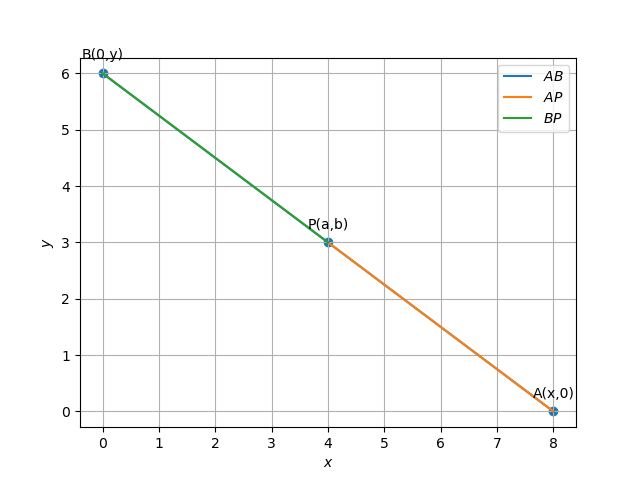
\includegraphics[width=\columnwidth]{chapters/11/10/2/18/figs/line1}
	\end{center}
\caption{}
\label{fig:11/10/2/18Fig1}
\end{figure}
Given that
\begin{align}
	\vec{P}&=\frac{\vec{A}+\vec{B}}{2}=\frac{x\vec{e_{1}}+y\vec{e_{2}}}{2}\\
\implies 	2\vec{P}&=x\vec{e_{1}}+y\vec{e_{2}}\\
	\vec{e_{1}}^{\top}\brak{2\vec{P}}&=\vec{e_{1}^{\top}}\brak{x\vec{e_{1}}+y\vec{e_{2}}}
=x\\				 
	\text{ and }\vec{e_{2}}^{\top}\brak{2\vec{P}}&=\vec{e_{2}^{\top}}\brak{x\vec{e_{1}}+y\vec{e_{2}}}
=y				 
\end{align}
Thus,
\begin{align}
	x&=2\vec{e_{1}}^{\top}\vec{P}=2a\\
	y&=2\vec{e_{2}}^{\top}\vec{P}=2b
\end{align}
yielding
\begin{align}
	\vec{A} &= 2a\vec{e_{1}}
	\vec{B} &= 2b\vec{e_{1}}
\end{align}
Thus, the direction vector of the line is 
\begin{align}
	\vec{m} &= \vec{A}-\vec{B}\\
	&=\myvec{a \\ -b}
\end{align}
and the normal vector is
\begin{align}
	\vec{n} = \myvec{b \\ a}
\end{align}
The equation of line passing through $\vec{P}$ is then obtained as
\begin{align}
	\vec{n}^{\top} \brak{\vec{x}-\vec{P}} &= 0\\
	\myvec{b & a}\vec{x} &= 2ab.
\end{align}



\item Find the equation of the set of points which are equidistant from the points $(1,2,3)$ and $(3,2,-1)$.
\item Find the equation of the set of points $P$, the sum of whose distances from $A(4,0,0)$ and $B(-4,0,0)$ is equal to $10$.
\item If $A=\myvec
{0 & -\tan \frac{\alpha}{2} \\ \tan \frac{\alpha}{2} & 0}$  and $I$ is the identity matrix of order $2$, show that $I+A= (I-A) \myvec
{\cos \alpha & -\sin \alpha \\ \sin \alpha & \cos \alpha}$.
\item Find the values of $\theta$ and $p$, if the equation $x \cos \theta + y \sin \theta = p$ is the normal form of the line $\sqrt 3x+y+2=0$.
\item Find the image of the point $(3,8)$ with respect to the line $x+3y=7$ assuming the line to be a plane mirror.
\end{enumerate}
